\documentclass[11pt]{article}

\usepackage[a4paper, total={6in, 8in}]{geometry}
\usepackage{graphicx,multirow,multicol}

\title{July2023 CSE300 Week9 Online Evaluation}
\author{2005ABC}
\date{\today}

\begin{document}
    \maketitle
    \section*{DNA vs RNA Comparison}
    \begin{table}[h]
        \centering
        \begin{tabular}{c|c}
             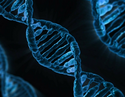
\includegraphics[]{images/DNA.png}&
            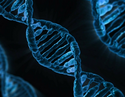
\includegraphics[]{images/DNA.png}\\
               Deoxyribonucleic acid& 
                Ribonucleic acid\\
         \end{tabular}
        \label{tab:my_label}
    \end{table}
    \section*{SPEC CPU Benchmark}
    \begin{table}[h]
        \centering
        \caption{SPECINTC2006 benchmark programs.}
        \begin{tabular}{|c|c|c|c|}
            \hline
             \multirow{2}{*}{Name}&\multicolumn{3}{c|}{Details}\\
             \cline{2-4}
             &Description&Instruction Count&Reference Time\\
             \hline
             gcc&GNU C Compiler&794 G&8050 sec\\
             \hline
             h264avc&Video Compression&3793 G&22130 sec\\
             \hline
        \end{tabular}
        \label{tab:my_label}
        \\This table is taken from \cite{vidref}
    \end{table}
    
    

    Table 1 shows some of the SPEC CPU benchmark programs that we can use to assess
the execution performance of different computational processors.
\pagebreak

    \section*{Newton’s Law of Universal Gravitation}
    Newton’s law of universal gravitation states that any two particles in this universe attract
each other with a force that is proportional to the product of their masses and inversely
proportional to the square of the distance between their centers. This is one of the foundational laws in classical physics that was first described and formulated in Sir Isaac Newton’s
famous Principia book \cite{newtbook}

The equation takes the form $F_g=G\frac{m_1m_2}{r^2}$ or $F_{ab}=-G\frac{m_am_b}{|r_{ab}|^2}$ among many other forms.

\section*{Display This Section Too!}
You need to display this section in your output PDF file. This section contains information
that may help you prepare the bibliography section.

\begin{enumerate}
    \item Citation about SPEC CPU Benchmark
    \begin{itemize}
        \item Authors: David A. Patterson, John L. Hennessy
        \item Title: Computer Organization and Design MIPS Edition
        \item Publisher: Morgan Kaufmann
        \item Year: 2013
        \item Edition: 5th
    \end{itemize}
    \item Citation about Universal Gravitation
    \begin{itemize}
        \item Authors: Isaac Newton
        \item Title: Philosophiae Naturalis Principia Mathematica
        \item Publisher: Jussu Societatis Regiae ac Typis Josephi Streater
        \item Year: 1687
    \end{itemize}
\end{enumerate}

\bibliographystyle{plain}
\bibliography{sample}
    
\end{document}